\begin{figure}[htb]
    % \vspace{-0.1cm}
    \begin{center}
    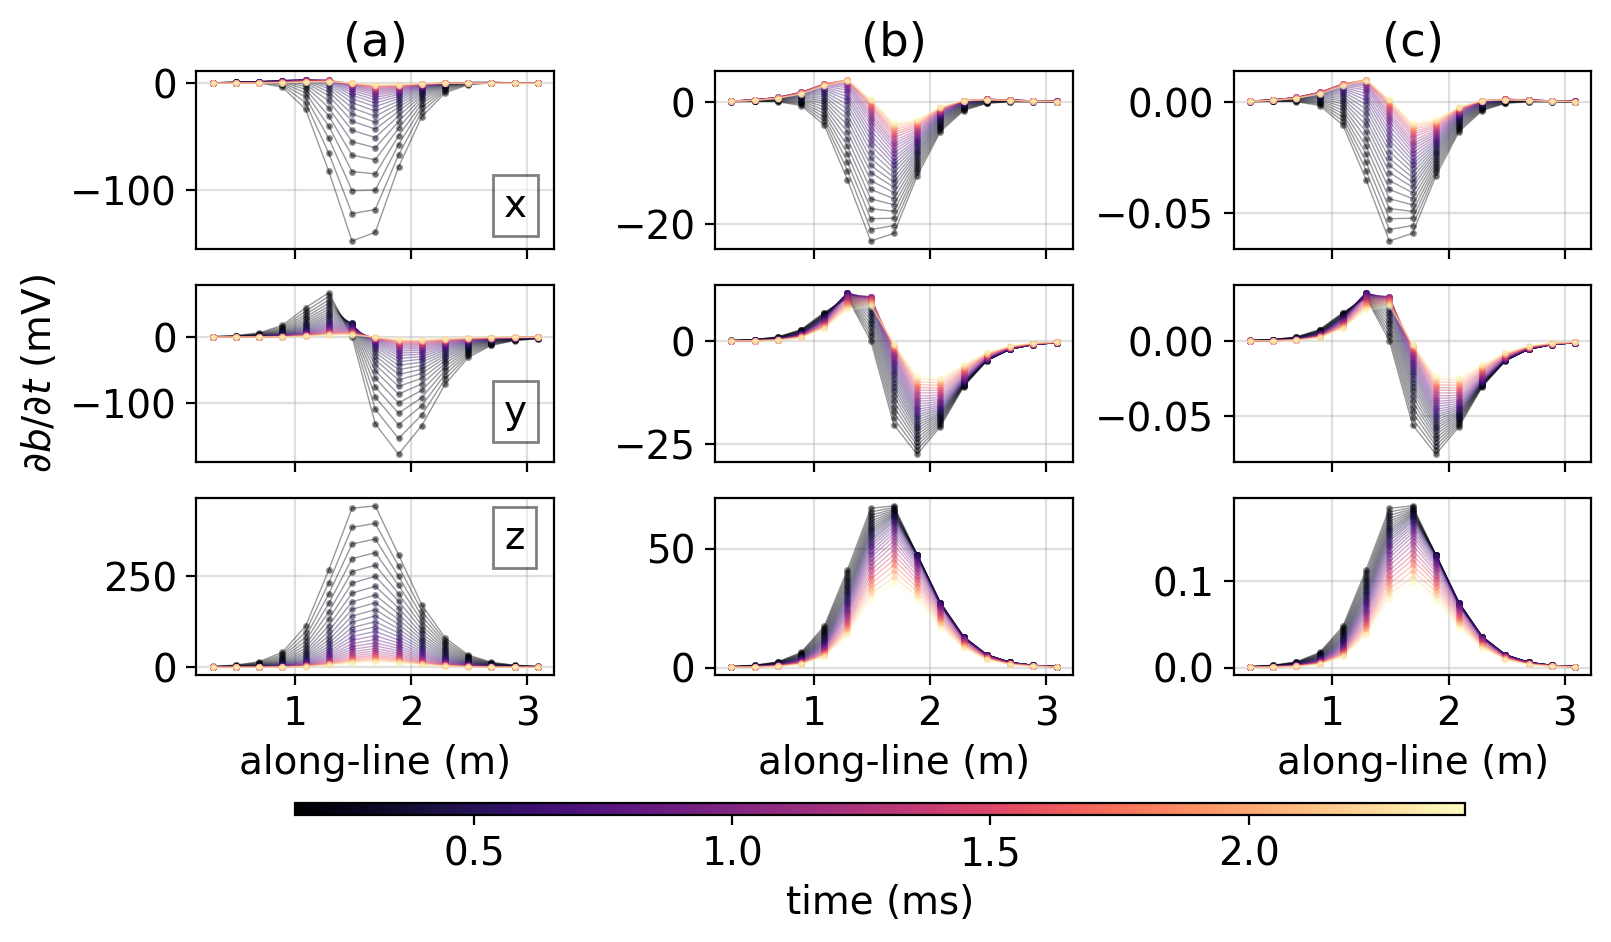
\includegraphics[width=\columnwidth]{figures/data_normalizations.png}
    \end{center}
    % \vspace{-0.5cm}
\caption{
    Subset of (a) simulated data,
    (b) data that have been multiplied by $t$, the time-channel (step 1 in the normalizations),
    (c) data from (b) which have been normalized by the maximum amplitude across all 165 inputs.
}
\label{fig:data-normalizations}
% \vspace{-0.1cm}
\end{figure}

